\documentclass{journal}
\usepackage{graphicx}
\usepackage{siunitx}
\usepackage{booktabs}



\begin{document}
\title{AP Calculus Final Project}
\author{Joshua Morin-Baxter, Alan Zhu, Nathan Wiley, and George Hong}
\date{\today}

\maketitle

\begin{abstract}
This is an analysis of data taken from the GOSH Flight Path Predictor\textsuperscript{TM}.
Four separate sets of data were analyzed:
temperature vs. density, wind velocity vs. pressure, wind angle vs. wind velocity, and wind velocity vs. altitude.
Each is discussed in more depth in subsequent parts.
\end{abstract}

\part{Wind Velocity Vs. Altitude}
This data has several interesting patterns.  Most notably, there appears to be an absolute maximum
slightly after 1000 feet, as can be seen in Figure \ref{josh1}.  At this point
the wind speed is nearly 40\si{\frac{m}{s}}.  Wind speed increases as it approaches
this maximum, though it increases at a slower and slower rate.
After the maximum, the wind speed begins to decrease at an increasing rate.
The question generated by this feature is, of course,
what atmospheric feature is responsible for this pattern?
A numerical analysis reveals more specific information:

% Please add the following required packages to your document preamble:
\begin{table}[]
\centering
\caption{My caption}
\label{my-label}
\begin{tabular}{@{}llllll@{}}
\toprule
altitude (m) & wind speed (m/s) & first derivative & second    & f is & concave \\ \midrule
947.84       & 5.90581712       &                  &           &      &         \\
985.55       & 6.1990502        & 0.007776003      &           & +    &         \\
1023.37      & 6.39453892       & 0.005168924      & -6.89E-05 & +    & DOWN    \\
1061.3       & 6.49228328       & 0.002576967      & -6.83E-05 & +    & DOWN    \\
1101.25      & 6.49228328       & 0                & -6.45E-05 & -    & DOWN    \\
1141.34      & 6.49228328       & 0                & 0         & -    & DOWN    \\
1182.52      & 6.59002764       & 0.002373588      & 5.76E-05  & +    & UP      \\
1224.81      & 6.59002764       & 0                & -5.61E-05 & -    & DOWN    \\
1268.21      & 6.59002764       & 0                & 0         & -    & DOWN    \\
1313.71      & 6.59002764       & 0                & 0         & -    & DOWN    \\
1361.33      & 6.59002764       & 0                & 0         & -    & DOWN    \\
1411.1       & 6.59002764       & 0                & 0         & -    & DOWN    \\
1463.04      & 6.49228328       & -0.001881871     & -3.62E-05 & -    & DOWN    \\
1518.18      & 6.49228328       & 0                & 3.41E-05  & -    & UP      \\
1575.56      & 6.47684996       & -0.000268967     & -4.69E-06 & -    & DOWN    \\
1639.2       & 6.47684996       & 0                & 4.23E-06  & -    & UP      \\
1710.22      & 6.3791056        & -0.001376293     & -1.94E-05 & -    & DOWN    \\
1792.78      & 6.3791056        & 0                & 1.67E-05  & -    & UP      \\
1889.17      & 6.26592792       & -0.001174164     & -1.22E-05 & -    & DOWN    \\
2000.74      & 6.26592792       & 0                & 1.05E-05  & -    & UP      \\
2130.05      & 6.15275024       & -0.000875243     & -6.77E-06 & -    & DOWN    \\
2277.72      & 5.41709532       & -0.004981749     & -2.78E-05 & -    & DOWN    \\
2447.89      & 3.54451916       & -0.01100415      & -3.54E-05 & -    & DOWN    \\
2641.95      & 2.81400868       & -0.003764354     & 3.73E-05  & -    & UP      \\
2861.54      & 5.82350608       & 0.013705075      & 7.96E-05  & +    & UP      \\
3107.44      & 9.14681432       & 0.013514877      & -7.73E-07 & +    & DOWN    \\
3381.51      & 15.16066468      & 0.021942753      & 3.08E-05  & +    & UP      \\
3681.25      & 18.38622856      & 0.010761206      & -3.73E-05 & +    & DOWN    \\
4002.43      & 18.86980592      & 0.001505627      & -2.88E-05 & +    & DOWN    \\
4344.09      & 18.91610588      & 0.000135515      & -4.01E-06 & +    & DOWN    \\
4706.73      & 19.2144834       & 0.000822793      & 1.90E-06  & +    & UP      \\
5089.27      & 20.63434884      & 0.003711678      & 7.55E-06  & +    & UP      \\
5491.59      & 22.02849208      & 0.00346526       & -6.12E-07 & +    & DOWN    \\
5913.8       & 21.9153144       & -0.00026806      & -8.84E-06 & -    & DOWN    \\
6358.13      & 23.72615728      & 0.004075446      & 9.78E-06  & +    & UP      \\
6822.71      & 26.43213272      & 0.005824563      & 3.76E-06  & +    & UP      \\
7313.41      & 24.72932308      & -0.003470164     & -1.89E-05 & -    & DOWN    \\
7830.24      & 26.751088        & 0.003911857      & 1.43E-05  & +    & UP      \\
8382.36      & 29.10209708      & 0.004258149      & 6.27E-07  & +    & UP      \\
8972.84      & 33.18678244      & 0.006917568      & 4.50E-06  & +    & UP      \\
9591.32      & 36.33003528      & 0.005082222      & -2.97E-06 & +    & DOWN    \\
10215.39     & 37.811634        & 0.002374091      & -4.34E-06 & +    & DOWN    \\
10824.28     & 39.2006328       & 0.002281198      & -1.53E-07 & +    & DOWN    \\
11416.76     & 39.18519948      & -2.60E-05        & -3.89E-06 & -    & DOWN    \\
11995.67     & 36.77760156      & -0.004158847     & -7.14E-06 & -    & DOWN    \\
12565.71     & 30.64028464      & -0.010766467     & -1.16E-05 & -    & DOWN    \\
13130.59     & 28.41788656      & -0.003934284     & 1.21E-05  & -    & UP      \\
13704.45     & 27.4970318       & -0.001604668     & 4.06E-06  & -    & UP      \\
14307.19     & 22.40918064      & -0.008441204     & -1.13E-05 & -    & DOWN    \\
14949.59     & 16.31301924      & -0.009489666     & -1.63E-06 & -    & DOWN    \\
15626.44     & 21.2722594       & 0.007326941      & 2.48E-05  & +    & UP      \\
16364.28     & 22.4040362       & 0.001533905      & -7.85E-06 & +    & DOWN    \\
17178.71     & 9.42461408       & -0.015936817     & -2.15E-05 & -    & DOWN    \\
18095.86     & 5.80292832       & -0.003948848     & 1.31E-05  & -    & UP      \\
19133.84     & 5.57142852       & -0.000223029     & 3.59E-06  & -    & UP      \\
20359.21     & 2.829442         & -0.00223768      & -1.64E-06 & -    & DOWN    \\
21888.32     & 2.55164224       & -0.000181674     & 1.34E-06  & -    & UP      \\
23904.7      & 0.20063316       & -0.001165955     & -4.88E-07 & -    & DOWN    \\
26910.97     & 0.31381084       & 3.76E-05         & 4.00E-07  & +    & UP      \\
33038.6      & 8.58607036       & 0.001349993      & 2.14E-07  & +    & UP      \\
AVG:         & 14.57059741      & 0.000699214      & -3.47E-06 & +    & DOWN    \\ \bottomrule
\end{tabular}
\end{table}

\begin{figure}
\centering
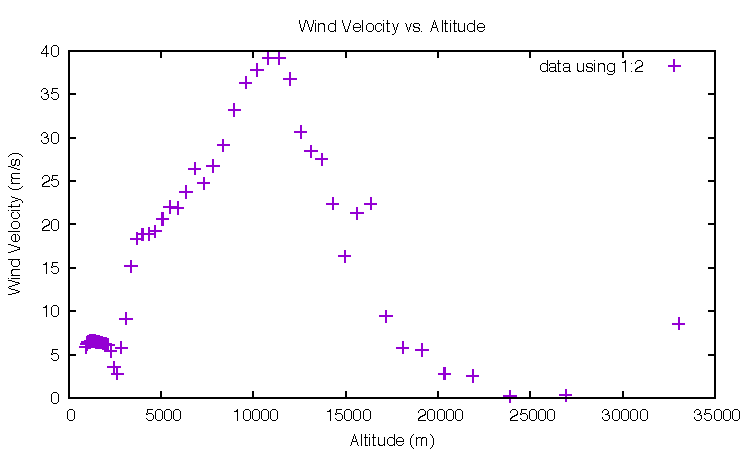
\includegraphics{josh-images/figure1.pdf}
\label{josh1}
\caption{Test}

\end{figure}


\part{Temperature Vs. Density}

\part{Wind Velocity vs. Pressure}

\part{Wind Angle vs. Wind Velocity}



\end{document}
